% Created 2018-12-23 dom 21:00
\documentclass[a4paper, 12pt]{article}
\usepackage[utf8]{inputenc}
\usepackage[T1]{fontenc}
\usepackage{fixltx2e}
\usepackage{graphicx}
\usepackage{longtable}
\usepackage{float}
\usepackage{wrapfig}
\usepackage{rotating}
\usepackage[normalem]{ulem}
\usepackage{amsmath}
\usepackage{textcomp}
\usepackage{marvosym}
\usepackage{wasysym}
\usepackage{amssymb}
\usepackage{hyperref}
\tolerance=1000
\usepackage[left=3cm, right=3cm, top=3.5cm, bottom=3.5cm]{geometry} % Márgenes recomendados
\usepackage{times} % La fuente debe ser Times New Romans
\usepackage[english, spanish, es-noshorthands, es-tabla]{babel}
\usepackage[spanish]{translator}
\usepackage[style=ieee, backend=biber]{biblatex} % Bibliografía en formato IEEE
\usepackage{sectsty}
\usepackage{portada}
\usepackage{listings}
\usepackage{xcolor}
\colorlet{punct}{red!60!black}
\definecolor{background}{HTML}{EEEEEE}
\definecolor{delim}{RGB}{20,105,176}
\colorlet{numb}{magenta!60!black}
\lstdefinelanguage{json}{
    basicstyle=\normalfont\ttfamily,
    numbers=left,
    numberstyle=\scriptsize,
    stepnumber=1,
    numbersep=8pt,
    showstringspaces=false,
    breaklines=true,
    frame=lines,
    backgroundcolor=\color{background},
    literate=
     *{0}{{{\color{numb}0}}}{1}
      {1}{{{\color{numb}1}}}{1}
      {2}{{{\color{numb}2}}}{1}
      {3}{{{\color{numb}3}}}{1}
      {4}{{{\color{numb}4}}}{1}
      {5}{{{\color{numb}5}}}{1}
      {6}{{{\color{numb}6}}}{1}
      {7}{{{\color{numb}7}}}{1}
      {8}{{{\color{numb}8}}}{1}
      {9}{{{\color{numb}9}}}{1}
      {:}{{{\color{punct}{:}}}}{1}
      {,}{{{\color{punct}{,}}}}{1}
      {\{}{{{\color{delim}{\{}}}}{1}
      {\}}{{{\color{delim}{\}}}}}{1}
      {[}{{{\color{delim}{[}}}}{1}
      {]}{{{\color{delim}{]}}}}{1},
}

\sectionfont{\MakeUppercase} % Las secciones deben estar en mayúsculas
\bibliography{\jobname}
\Director{Fernando Pérez Costoya}
%\Lugar{Bilbao} % Por omisión: Madrid
%\Grado{Graduado en Matemáticas e Informática} % Por omisión: Graduado en Ingeniería Informática
%\Trabajo{TRABAJO FIN DE MÁSTER} % Por omisión: TRABAJO FIN DE GRADO
\author{Carlos Sánchez Marín}
\date{Enero de 2019}
\title{Desarrollo de una solución nativa y multiplataforma para la interacción desde una plataforma móvil con una aplicación bancaria}
\hypersetup{
  pdfkeywords={},
  pdfsubject={},
  pdfcreator={Emacs 25.2.2 (Org mode 8.2.10)}}
\begin{document}

\maketitle
\begin{export}
\null
\newpage

\pagenumbering{roman} \% La numeración debe ser romana hasta la primera sección
\tableofcontents
\newpage

\listoffigures
\listoftables
\newpage
\end{export}

\begin{abstract}
\normalsize
Aquí el texto del abstract.

\textbf{Palabras clave:} palabra 1, palabra 2, palabra 3\ldots{}
\end{abstract}

\begin{otherlanguage}{english}
\begin{abstract}
\normalsize
Here goes the abstract text.

\textbf{Keywords:} keyword 1, keyword 2, keyword 3\ldots
\end{abstract}
\end{otherlanguage}

\newpage
\pagenumbering{arabic}% Iniciamos la numeración árabe en la primera sección

\section{Introducción}
\label{sec-1}
En los últimos años el sector bancario ha visto como los pagos con tarjetas ha crecido exponencialmente.
Según los datos ofrecidos por el Banco de España, desde 2002 hasta 2017 el número de operaciones creció
un 245\% y el importe de las operaciones un 188\%, llegando a un gasto total de 135.246,47 millones de €
en el 2017\cite{BancoEspana}.
\\
\\
Este rápido incremento de las operaciones con tarjeta también se ha trasladado al entorno corporativo,
generando nuevas necesidades para el control por parte de las empresas de las tarjetas que dan a sus
empleados. Con el objetivo de cubrir esta necesidad, tanto Mastercard \footnote{\url{https://developer.mastercard.com/product/spend-controls}} como Visa \footnote{\url{https://developer.visa.com/capabilities/vctc}} han
implementado nuevas funcionalidades de control de tarjetas que permiten el control directo por parte
de las empresas de sus tarjetas, de manera que se puedan recibir alertas de gasto o bloquear determinados tipos de pago.
\\
\\
Este servicio es ofrecido a través de diversas API REST y en Vipera hemos implementado una aplicación que
abstrae a los clientes finales (bancos y empresas) de las API proporcionadas por Visa y Mastercard,
ofreciendo una API REST centralizada que simplifica las operaciones. Esta API interactúa con un servicio
propietario de Vipera que integra toda la funcionalidad requerida por los distintos clientes finales.
\\
\\
Los SDK desarrollados para la integración de nuestro servicio en las aplicaciones móviles de los clientes
pretenden abstraer totalmente de las llamadas al servicio de manera que los desarrolladores tan solo
vean funciones totalmente descriptivas sin tener que preocuparse de la configuración necesaria para la
interacción. Así mismo, ya que la demo técnica realizada por Vipera está implementada con Ionic\footnote{\url{https://ionicframework.com/}},
se ha implementado un plugin de Cordova\footnote{\url{https://cordova.apache.org/}} que habilita la llamada a los SDK de iOS y Android.

\section{Estado del arte}
\label{sec-2}
\subsection{Tecnologías}
\label{sec-2-1}
En el mercado móvil actual iOS y Android lideran con mano de hierro dejando una cuota residual a otros
entornos como Windows Phone y otros sistemas menores. En conjunto, iOS y Android acapararon el 99,7\% de
las ventas en el primer trimestre de 2018 en España, dejando a Windows fuera de las estadísticas al no lograr
el 0,1\% de las ventas totales\footnote{\url{https://bit.ly/2Cu8NVy}}. Teniendo presentes estos datos, resulta obvio que cualquier tipo de desarrollo
fuera de Android e iOS tendría un impacto muy reducido y difícilmente sería rentable para cualquier aplicación
que no tenga como objetivo a todos los usuarios del mercado móvil.
\subsubsection{iOS}
\label{sec-2-1-1}
El sistema operativo iOS es un sistema propietario desarrollado por Apple\footnote{\url{https://apple.com/es/}} para sus dispositivos
móviles iPhone, iPad y iPod Touch. Fue presentado junto con el primer iPhone en junio de 2007. En un
principio Apple no iba a proporcionar SDK para desarrollo de aplicaciones nativas por parte de terceros,
pero ante la reacción negativa de todos los desarrolladores, Apple reconsideró su decisión y terminó
lanzando la primera versión del SDK en Marzo de 2008 junto a la segunda versión de iOS.
\\
\\
El SDK originalmente proporcionaba un acceso muy limitado a las funciones del sistema operativo,
además de tan solo proporcionar soporte para el lenguaje Objective-C\footnote{\url{https://developer.apple.com/library/archive/documentation/Cocoa/Conceptual/ProgrammingWithObjectiveC/Introduction/Introduction.html}}. Año tras año Apple ha
actualizado su sistema operativo móvil junto con el SDK aprovechando el lanzamiento de los nuevos iPhone.
\\
\\
En 2014, Apple lanzó Swift\footnote{\url{https://swift.org/}}, un nuevo lenguaje más moderno que sustituyó a Objective-C como
lenguaje de referencia para el desarrollo de aplicaciones iOS. No obstante, ambos lenguajes son actualmente
soportados por el SDK de Apple, aunque la documentación tan solo es actualizada para Swift.
\\
\\
\subsubsection{Android}
\label{sec-2-1-2}
Android\footnote{\url{https://www.android.com}} fue creado en 2003 como un fork del kernel de Linux para dispositivos
móviles. Inicialmente fue concebido como un sistema operativo móvil inteligente que
estuviese pendiente de la localización del usuario y sus preferencias. En 2005 la
empresa propietaria del sistema operativo fue comprada por Google, que se hizo cargo
del desarrollo. Dos años más tarde, Google hizo público el primer SDK en fase beta
para Android, que fue distribuido a desarrolladores y fabricantes de dispositivos
móviles. No fue hasta septiembre de 2008 que se lanzó al mercado el primer dispositivo
con Android.
\\
\\
Las primeras versiones del SDK proporcionado por Google contaban tan solo con
soporte para el lenguaje Java\footnote{\url{https://www.java.com}}. Al contrario de su principal competidor, el código fuente
de Android siempre ha sido open source\footnote{\url{https://source.android.com/}} lo que ha atraído a una gran cantidad de
desarrolladores y fabricantes. De todos modos, la práctica totalidad de los fabricantes
integran en sus terminales la versión de Android propietaria de Google, que incluye
integración con las apps de Google bajo la capa Google Play Services\footnote{\url{https://developers.google.com/android/guides/overview}}.
\\
\\
En el evento Google I/O de 2017, Google anunció de manera oficial que se añadía un
nuevo lenguaje soportado al SDK de Android \footnote{\url{https://blog.jetbrains.com/kotlin/2017/05/kotlin-on-android-now-official/}}, Kotlin\footnote{\url{https://kotlinlang.org/}}. Este lenguaje desarrollado
por la empresa Jetbrains\footnote{\url{https://www.jetbrains.com/}} funciona sobre la Java Virtual Machine, por lo que es totalmente compatible con el código Java y puede
coexistir con este en una misma aplicación.
\subsubsection{Cordova}
\label{sec-2-1-3}
En el año 2011, Adobe Systems\footnote{\url{https://www.adobe.com/}} compró la empresa Nitobi y renombró su producto
como Phonegap\footnote{\url{https://phonegap.com/}} . Así mismo, lanzó una versión open source del producto nombrada
Cordova que es mantenida por la Apache Software Foundation\footnote{\url{https://www.apache.org/}}.
Este framework permite el desarrollo de aplicaciones híbridas basadas en la web,
embebiendo una aplicación web dentro de una aplicación nativa para el sistema
operativo deseado. Esta solución se acerca a la idea que tenía Apple de aplicaciones
móviles en un principio, pero va más allá otorgando un sistema de plugins nativos que
permiten la interacción con el sistema operativo.
\\
\\
Los plugins proporcionan una implementación en código nativo (Objective-C para iOS
y Java para Android) que será invocada por un wrapper escrito en Javascript\footnote{\url{https://developer.mozilla.org/bm/docs/Web/JavaScript}}. En
tiempo de ejecución Cordova es capaz de saber sobre qué plataforma está ejecutándose
e invocar al código nativo de esta, con lo que abstrae a los desarrolladores de
aplicaciones de esta gestión y facilita la escritura de código.
\subsection{MOTIF}
\label{sec-2-2}
El despliegue del lado del servidor de la aplicación bancaria con la que se ha operado
para la realización de este trabajo está realizado sobre una plataforma propietaria propiedad
de Vipera\footnote{\url{http://www.vipera.com/}} cuyo nombre comercial es MOTIF\footnote{\url{http://www.vipera.com/motif}}.
\\
\\
MOTIF es un servicio desarrollado en Java haciendo uso del framework OSGi\footnote{\url{https://www.osgi.org/}}, creado en 1999
como una primera aproximación al mundo de los microservicios en Java. En concreto, el desarrollo de MOTIF
ha sido llevado a cabo empleando Apache Felix\footnote{\url{https://felix.apache.org/}} como implementación del framework OSGi. El uso de
este framework facilita la integración con los clientes finales, por lo general banco y otros servicios
financieros, ya que estos suelen emplear Java en sus propios servicios y la arquitectura OSGi permite una
integración sencilla de diferentes módulos a los que se llama \emph{plugins} con el resto del sistema. En la \hyperref[fig:motif-core]{figura 1}
se representan los servicios básicos implementados en el core de MOTIF.
\begin{figure}[htb]
\centering
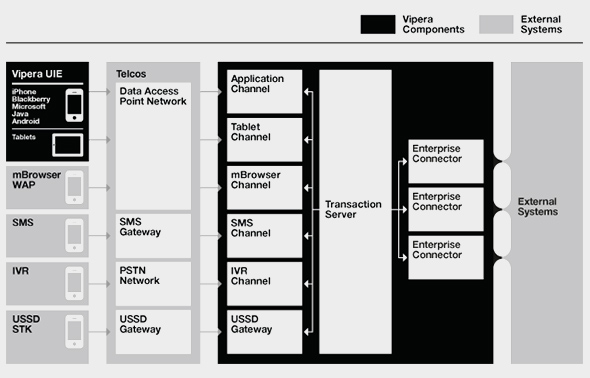
\includegraphics[width=.9\linewidth]{./images/motif.jpg}
\caption{\label{fig:motif-core}Diagrama de módulos predefinidos de MOTIF}
\end{figure}
\\
\\
En el caso concreto de la aplicación para la que se ha implentado la solución desarrollada como trabajo
fin de grado, se ha hecho uso de los plugins que conforman el core de MOTIF, además de distintos plugins que
permiten la interacción con los servicios de Mastercard y VISA, así como plugins de persistencia de datos empleando
la librería Hibernate\footnote{\url{https://hibernate.org/}} y otros que implementan toda la lógica de negocio, que será explicada más adelante.
\\
\\
Para realizar la conexión con MOTIF, por defecto existen 2 métodos distintos:
\begin{itemize}
\item \textbf{API REST}: Está pensada para dar servicio a implementaciones de administracióndel sistema como podría ser un Help Desk.
\item \textbf{JSON Protocol}: Este método de conexión es el que se emplea en las soluciones móviles. Se basa en peticiones POST a un endpoint estático, el cual procesa la información enviada en la petición y determina el comportamiento que debe seguir el servidor.
\end{itemize}

\subsection{Modos de conexión con MOTIF}
\label{sec-2-3}
\subsubsection{Peticiones POST}
\label{sec-2-3-1}
La forma más básica de hacer llamadas al endpoint JSON de MOTIF es la construcción de peticiones POST haciendo uso
de aplicaciones como Postman\footnote{\url{https://www.getpostman.com/}} o empleando directamente las librerías HTTP de los distintos lenguajes.
El siguiente código es un ejemplo del cuerpo de una llamada a MOTIF.
\\
\begin{lstlisting}[language=json]
{
  "req" : {
        "dom" : "{{domain}}",
        "app" : "{{application}}",
        "srv" : "{{service}}",
        "op"  : "{{operation}}",
        "header" :
        {
            "user":"user1@company1.com",
            "otp":"123456",
            "private:pwd":"1111",
            "private:vpwd":"1111",
            "email": "user1@company1.com"
        }
    }
}
\end{lstlisting}
\\
Como se puede apreciar, todos los campos de la llamada están encapsulados dentro del parámetro \emph{req}, el cual
es interceptado por el endpoint JSON de MOTIF. Una vez se ha interceptado la llamada, MOTIF comprueba los campos
\emph{dom} (dominio al que se está llamando), \emph{app} (aplicación del dominio), \emph{srv} (servicio de la aplicación) y \emph{op}
(operación del servicio).
\\
\\
Por último, en el campo \emph{header} se encontrarán contenidos los parametros requeridos por la operación. En este caso
se trata de una llamada de ejemplo para la activación de usuarios, por lo que se pasan como parámetros el usuario,
OTP (One Time Password), contraseña y su verificación y el email del usuario. Cabe destacar que los campos ligados a
la contraseña tienen el prefijo \emph{private}, el cual al ser detectado por MOTIF le indica que no debe quedar constancia
en los logs de esos campos.
\section{Otra sección}
\label{sec-3}

\subsection{Una subsección}
\label{sec-3-1}

\subsection{Otra subsección}
\label{sec-3-2}

\section{Resultados y conclusiones}
\label{sec-4}

\subsection{Pruebas}
\label{sec-4-1}

\subsection{Conclusiones}
\label{sec-4-2}

\printbibliography[heading=bibnumbered] % Última sección, numerada, para la bibliografía
% Emacs 25.2.2 (Org mode 8.2.10)
\end{document}
